%% Chapter 2: Modeling Physical Systems
%% IEEE-Formatted Control Systems Textbook
%% Self-contained chapter with complete derivations and practical experiments

\chapter{Modeling Physical Systems}
\label{ch:modeling}

\begin{quote}
\textit{``The purpose of computing is insight, not numbers.''} --- Richard Hamming
\end{quote}

\section{Historical Motivation: The Need to Predict Before Building}

The ability to predict how a physical system will behave---before constructing it---represents one of humanity's greatest intellectual achievements. This section traces the development of mathematical modeling from Newton's mechanics through the analog computers of the Victorian era to modern digital simulation.

\subsection{Newton's Laws of Motion (1687): The Birth of Mathematical Physics}

In 1687, Isaac Newton published \textit{Philosophi\ae{} Naturalis Principia Mathematica}, fundamentally transforming our understanding of the physical world. Newton's revolutionary insight was that the motion of all objects---from falling apples to orbiting planets---could be described by three simple mathematical laws.

The Second Law, expressed mathematically as
\begin{equation}
\mathbf{F} = m\mathbf{a} = m\frac{d^2\mathbf{x}}{dt^2},
\label{eq:newton2}
\end{equation}
established the differential equation as the language of physics. This was not merely an academic exercise; Newton needed these tools to explain Kepler's laws of planetary motion and the phenomenon of tides.

The profound implication was this: if one knew the forces acting on a body and its initial conditions (position and velocity), one could predict its future trajectory with mathematical certainty. This was the first ``system model''---a mathematical description that captured the essential physics of motion.

Newton's work raised a compelling question: could this same approach be applied to predict the behavior of engineered systems? The answer, developed over the following centuries, would prove essential to the Industrial Revolution and beyond.

\subsection{Kirchhoff's Circuit Laws (1845): Extending Models to Electricity}

Gustav Kirchhoff, a German physicist, recognized that electrical circuits followed conservation principles analogous to those in mechanics. In 1845, at just 21 years old, Kirchhoff formulated his circuit laws:

\textbf{Kirchhoff's Current Law (KCL):} The algebraic sum of currents entering any node equals zero:
\begin{equation}
\sum_{k=1}^{n} i_k = 0.
\end{equation}

\textbf{Kirchhoff's Voltage Law (KVL):} The algebraic sum of voltages around any closed loop equals zero:
\begin{equation}
\sum_{k=1}^{n} v_k = 0.
\end{equation}

These laws, combined with the constitutive relationships for resistors, inductors, and capacitors, enabled the systematic derivation of differential equations describing electrical network behavior. For the first time, engineers could analyze complex electrical systems before building them.

The telegraph industry, rapidly expanding in the 1840s-1860s, provided the economic motivation. Laying submarine cables across the Atlantic was extraordinarily expensive (the first successful transatlantic cable in 1866 cost approximately \$12 million in contemporary dollars). Mathematical modeling allowed engineers to predict signal degradation and design appropriate compensation before committing to construction.

\subsection{Lord Kelvin's Mechanical Analog Computers (1870s)}

William Thomson (later Lord Kelvin) recognized that differential equations appeared across many domains of physics and engineering. His insight: build mechanical devices that solve differential equations by physical analogy.

In 1876, Kelvin constructed his famous \textbf{tide-predicting machine}, a mechanical analog computer using pulleys, gears, and cables to sum harmonic components of tidal motion. The device could predict tide heights for any harbor, years into the future, by physically implementing the Fourier series:
\begin{equation}
h(t) = h_0 + \sum_{n=1}^{N} A_n \cos(\omega_n t + \phi_n),
\end{equation}
where each term corresponded to a specific astronomical influence (lunar, solar, etc.).

\begin{figure}[htbp]
\centering
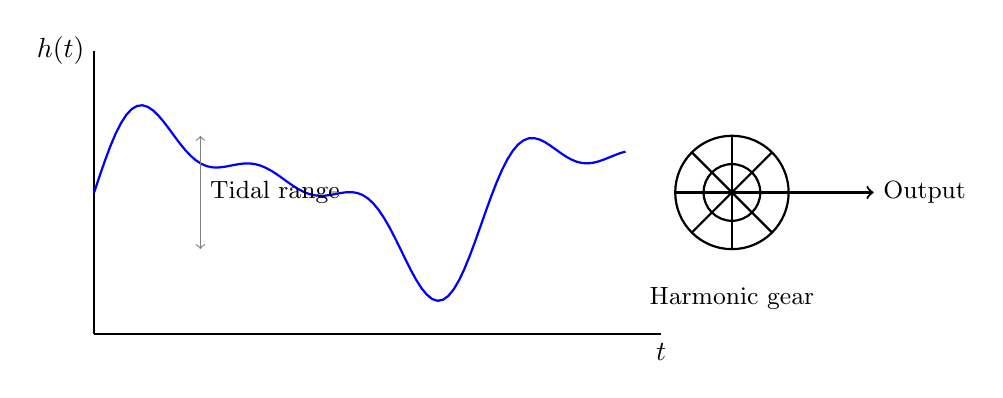
\begin{tikzpicture}[scale=0.9]
% Tide predictor conceptual diagram
\draw[thick] (0,0) -- (8,0);
\draw[thick] (0,0) -- (0,4);
\node[left] at (0,4) {$h(t)$};
\node[below] at (8,0) {$t$};

% Draw tide curve
\draw[blue, thick, domain=0:7.5, samples=100]
    plot (\x, {2 + 0.8*sin(60*\x) + 0.5*sin(130*\x) + 0.3*sin(200*\x)});

% Annotations
\draw[<->, gray] (1.5,1.2) -- (1.5,2.8);
\node[right, font=\small] at (1.5,2) {Tidal range};

% Gear representation
\draw[thick] (9,2) circle (0.8);
\draw[thick] (9,2) circle (0.4);
\foreach \angle in {0,45,...,315} {
    \draw[thick] (9,2) -- +(\angle:0.8);
}
\node[below, font=\small] at (9,0.8) {Harmonic gear};

\draw[->, thick] (9.8,2) -- (11,2);
\node[right, font=\small] at (11,2) {Output};
\end{tikzpicture}
\caption{Conceptual representation of Kelvin's tide-predicting machine. Gears rotating at different frequencies (corresponding to astronomical periods) are summed mechanically to produce the tide prediction.}
\label{fig:tide_predictor}
\end{figure}

This was perhaps the first example of ``simulation''---using one physical system (the mechanical computer) to model another (ocean tides). The machine remained in use by the British Admiralty until the 1960s, demonstrating the enduring value of accurate physical models.

\subsection{Heaviside's Operational Calculus (1880s-1890s)}

Oliver Heaviside, a self-taught English electrical engineer, faced a practical problem: analyzing the propagation of electrical signals through long telegraph cables. The partial differential equations governing transmission lines (derived from Maxwell's equations) were notoriously difficult to solve.

Heaviside developed ``operational calculus,'' treating the differentiation operator $d/dt$ as an algebraic quantity $p$. Differential equations became algebraic equations:
\begin{equation}
\text{If } p \equiv \frac{d}{dt}, \quad \text{then } L\frac{di}{dt} + Ri = v(t) \quad \Rightarrow \quad (Lp + R)i = v.
\end{equation}

This revolutionary simplification allowed engineers to solve complex circuit problems by algebraic manipulation. Although mathematicians initially dismissed Heaviside's methods as lacking rigor, his techniques worked remarkably well in practice. The formal justification came later through Laplace transform theory, which we shall study in Chapter~\ref{ch:transfer_functions}.

Heaviside's work on transmission lines led to the discovery of the ``distortionless line'' condition:
\begin{equation}
\frac{R}{L} = \frac{G}{C},
\end{equation}
where $R$, $L$, $G$, and $C$ are the resistance, inductance, conductance, and capacitance per unit length. This insight, derived purely from mathematical modeling, enabled the design of long-distance telephone and telegraph lines that transmitted signals without distortion.

\subsection{The Cost of Not Modeling: Engineering Disasters}

The 19th and early 20th centuries provided tragic demonstrations of what happens when engineers build without adequate mathematical models.

\textbf{The Tacoma Narrows Bridge (1940):} This suspension bridge in Washington State collapsed just four months after opening, due to aeroelastic flutter---a dynamic instability caused by the interaction between wind forces and structural motion. The designers had modeled static loads but not the dynamic, frequency-dependent behavior that proved fatal. The disaster catalyzed the development of aeroelasticity as a rigorous engineering discipline.

\textbf{The de Havilland Comet (1954):} The world's first commercial jet airliner suffered a series of catastrophic mid-flight breakups. Investigation revealed that the square-cornered windows created stress concentrations, and repeated pressurization cycles caused metal fatigue. The failure to model cyclic stress behavior cost 56 lives and nearly destroyed the British commercial aviation industry.

These disasters underscored a fundamental truth: \textit{mathematical models are not optional luxuries but essential tools for predicting and preventing failure}. Modern engineering ethics require modeling and simulation before any safety-critical system is built.

\subsection{The Evolution to Digital Simulation}

The electronic analog computers of the 1940s-1960s used operational amplifiers, resistors, and capacitors to physically implement differential equations. Each coefficient in the equation corresponded to a component value that could be adjusted. Engineers could ``simulate'' a system by building an electronic circuit with the same mathematical structure.

The transition to digital computers in the 1970s and beyond enabled more complex simulations and eliminated the analog computer's sensitivity to component drift. Today, software tools like MATLAB/Simulink, Python with SciPy, and specialized packages enable engineers to simulate systems of virtually unlimited complexity.

Yet the fundamental principle remains unchanged from Newton's time: derive differential equations from physical laws, solve them (analytically or numerically), and use the solutions to predict system behavior. This is the essence of mathematical modeling.


\section{Modern Applications of Physical System Models}

The mathematical techniques developed centuries ago now underpin virtually every engineered system. This section highlights contemporary applications across diverse fields.

\subsection{Digital Twins in Manufacturing}

A \textbf{digital twin} is a virtual replica of a physical system that is continuously updated with real-time sensor data. The concept, pioneered in aerospace (NASA used digital twins for Apollo 13 contingency planning), has now spread to manufacturing, power systems, and infrastructure.

Consider a digital twin of a CNC milling machine. The model includes:
\begin{itemize}
\item Mechanical dynamics: motor inertias, gearbox ratios, structural compliance
\item Thermal effects: spindle heating, thermal expansion of workpiece
\item Cutting forces: empirical models relating material properties to forces
\item Wear models: tool degradation as a function of cutting time and conditions
\end{itemize}

By comparing predicted behavior (from the model) with measured behavior (from sensors), deviations can be detected that indicate impending failure or quality problems. This ``model-based diagnostics'' approach can predict tool breakage hours before it occurs, preventing costly damage and downtime.

\subsection{Vehicle Dynamics Simulation}

Modern vehicles are developed through extensive simulation before physical prototypes are built. A vehicle dynamics model might include:
\begin{itemize}
\item \textbf{Chassis dynamics:} sprung and unsprung masses, suspension geometry
\item \textbf{Tire models:} the Pacejka ``magic formula'' relating slip to force
\item \textbf{Powertrain:} engine torque curves, transmission dynamics
\item \textbf{Driver models:} for closed-loop evaluation of handling
\end{itemize}

The differential equations governing a vehicle can exceed thousands of states when detailed subsystem models are included. Yet the fundamental approach---derive equations from physics, solve them numerically---remains the same as in Newton's era.

\subsection{HVAC System Modeling}

Heating, ventilation, and air conditioning (HVAC) systems represent a compelling control problem: maintain comfortable temperature and humidity while minimizing energy consumption. Mathematical models enable:
\begin{itemize}
\item \textbf{Load prediction:} how will the building temperature evolve given weather forecasts?
\item \textbf{Optimal control:} model predictive control (MPC) can pre-cool buildings during off-peak hours
\item \textbf{Fault detection:} deviations from model predictions indicate sensor faults or equipment degradation
\end{itemize}

Building thermal models typically use lumped-parameter (RC network) representations, where resistances represent insulation and capacitances represent thermal mass. These models are directly analogous to electrical circuits, demonstrating the power of the electrical-thermal analogy.

\subsection{Pharmacokinetics: Modeling Drug Dynamics in the Body}

Pharmacokinetic models describe how drugs are absorbed, distributed, metabolized, and excreted (ADME) in the body. A simple one-compartment model treats the body as a well-mixed tank:
\begin{equation}
V\frac{dC}{dt} = -k_e V C + R(t),
\end{equation}
where $C$ is drug concentration, $V$ is volume of distribution, $k_e$ is elimination rate constant, and $R(t)$ is the rate of drug administration.

These models are essential for:
\begin{itemize}
\item Determining dosing schedules that maintain therapeutic concentrations
\item Predicting drug interactions
\item Designing controlled-release formulations
\end{itemize}

The parallel to engineering control systems is striking: the ``plant'' is the human body, the ``input'' is drug dosage, and the ``output'' is blood concentration. Feedback control concepts, including proportional-integral controllers for automated drug delivery, are increasingly common in medical devices.


\section{Mathematical Foundation: Deriving Differential Equations from Physics}

We now develop the systematic approach to deriving differential equations that describe physical systems. The key insight is that physical laws (conservation of energy, momentum, charge, etc.) combined with constitutive relationships (describing material properties) yield differential equations that govern system dynamics.

\subsection{Newton's Second Law: The Foundation of Mechanical Systems}

Newton's Second Law states that the net force on a body equals its mass times acceleration:
\begin{equation}
\sum F = ma = m\frac{d^2x}{dt^2} = m\ddot{x}.
\label{eq:newton_basic}
\end{equation}

We use the overdot notation $\dot{x} \equiv dx/dt$ and $\ddot{x} \equiv d^2x/dt^2$ throughout this text.

\subsubsection{The Mass-Spring-Damper System: A Complete Derivation}

Consider the canonical mechanical system shown in Fig.~\ref{fig:msd_fbd}: a mass $m$ connected to a fixed support by a spring (stiffness $k$) and a viscous damper (damping coefficient $b$), with an external force $F(t)$ applied.

\begin{figure}[htbp]
\centering
\begin{tikzpicture}[scale=1.0]
% Ground
\fill[pattern=north east lines] (-0.5,0) rectangle (4.5,0.3);
\draw[thick] (-0.5,0) -- (4.5,0);

% Spring
\draw[thick] (0,0) -- (0,-0.5);
\draw[thick, decorate, decoration={zigzag, segment length=4, amplitude=3}]
    (0,-0.5) -- (0,-2.5);
\draw[thick] (0,-2.5) -- (0,-3);
\node[left] at (-0.3,-1.5) {$k$};

% Damper
\draw[thick] (2,0) -- (2,-0.8);
\draw[thick] (1.7,-0.8) rectangle (2.3,-1.2);
\draw[thick] (2,-1.2) -- (2,-2.3);
\draw[thick] (1.6,-2.3) -- (2.4,-2.3);
\draw[thick] (2,-2.3) -- (2,-3);
\node[right] at (2.5,-1.5) {$b$};

% Mass
\draw[thick, fill=gray!30] (-0.5,-3) rectangle (2.5,-4);
\node at (1,-3.5) {$m$};

% Position reference
\draw[dashed] (3,-3) -- (4,-3);
\draw[<->] (3.5,-3) -- (3.5,-4.5);
\node[right] at (3.5,-3.75) {$x$};

% Equilibrium reference
\draw[dashed, gray] (-1,-3) -- (-0.6,-3);
\node[left, gray] at (-1,-3) {$x=0$};

% External force
\draw[->, ultra thick, red] (1,-4) -- (1,-5.5);
\node[right, red] at (1,-5) {$F(t)$};
\end{tikzpicture}
\caption{Mass-spring-damper system. The position $x$ is measured from the equilibrium position where the spring is at its natural length.}
\label{fig:msd_fbd}
\end{figure}

\textbf{Step 1: Define Coordinates and Sign Conventions}

Let $x$ denote the displacement of the mass from its equilibrium position, with positive $x$ defined downward. We measure from equilibrium so that gravity effects are already accounted for by the static spring deflection.

\textbf{Step 2: Draw the Free Body Diagram}

Isolating the mass, we identify all forces acting on it:
\begin{itemize}
\item \textbf{Spring force:} By Hooke's Law, the spring exerts a restoring force proportional to displacement: $F_{\text{spring}} = -kx$. The negative sign indicates the force opposes displacement.
\item \textbf{Damping force:} The viscous damper exerts a force proportional to velocity: $F_{\text{damper}} = -b\dot{x}$. The negative sign indicates the force opposes motion.
\item \textbf{Applied force:} The external force $F(t)$ acts on the mass.
\end{itemize}

\begin{figure}[htbp]
\centering
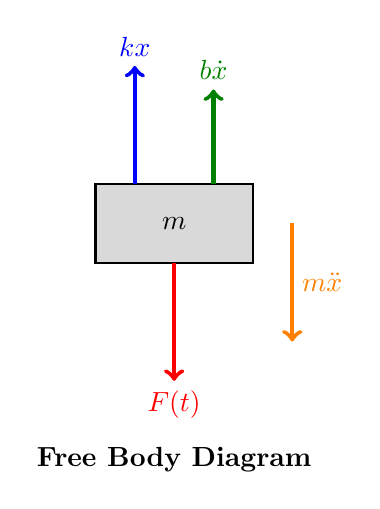
\begin{tikzpicture}[scale=1.0]
% Mass (isolated)
\draw[thick, fill=gray!30] (0,0) rectangle (2,1);
\node at (1,0.5) {$m$};

% Spring force
\draw[->, ultra thick, blue] (0.5,1) -- (0.5,2.5);
\node[above, blue] at (0.5,2.5) {$kx$};

% Damping force
\draw[->, ultra thick, green!50!black] (1.5,1) -- (1.5,2.2);
\node[above, green!50!black] at (1.5,2.2) {$b\dot{x}$};

% Applied force
\draw[->, ultra thick, red] (1,0) -- (1,-1.5);
\node[below, red] at (1,-1.5) {$F(t)$};

% Acceleration
\draw[->, ultra thick, orange] (2.5,0.5) -- (2.5,-1);
\node[right, orange] at (2.5,-0.25) {$m\ddot{x}$};

\node at (1,-2.5) {\textbf{Free Body Diagram}};
\end{tikzpicture}
\caption{Free body diagram of the mass showing all forces.}
\label{fig:fbd}
\end{figure}

\textbf{Step 3: Apply Newton's Second Law}

Summing forces in the positive $x$ direction:
\begin{equation}
\sum F = ma \quad \Rightarrow \quad F(t) - kx - b\dot{x} = m\ddot{x}.
\end{equation}

\textbf{Step 4: Rearrange into Standard Form}

The standard form places all terms involving the dependent variable on the left and the input on the right:
\begin{equation}
\boxed{m\ddot{x} + b\dot{x} + kx = F(t)}
\label{eq:msd_ode}
\end{equation}

This is a second-order, linear, ordinary differential equation (ODE) with constant coefficients. The order of the equation (second) corresponds to the number of energy storage elements in the system: kinetic energy in the mass and potential energy in the spring.

\subsubsection{Standard Parameters: Natural Frequency and Damping Ratio}

Dividing Eq.~\eqref{eq:msd_ode} by $m$ yields:
\begin{equation}
\ddot{x} + \frac{b}{m}\dot{x} + \frac{k}{m}x = \frac{F(t)}{m}.
\end{equation}

We define two fundamental parameters:
\begin{itemize}
\item \textbf{Natural frequency:} $\omega_n = \sqrt{k/m}$ [rad/s]
\item \textbf{Damping ratio:} $\zeta = \frac{b}{2\sqrt{km}} = \frac{b}{2m\omega_n}$ [dimensionless]
\end{itemize}

The equation becomes:
\begin{equation}
\boxed{\ddot{x} + 2\zeta\omega_n\dot{x} + \omega_n^2 x = \frac{F(t)}{m}}
\label{eq:msd_standard}
\end{equation}

This \textbf{standard second-order form} appears throughout control systems engineering. The parameters $\omega_n$ and $\zeta$ completely characterize the system's dynamic behavior, as we shall explore in Chapter~\ref{ch:first_second_order}.

\subsection{Electrical Systems: RLC Circuits from Kirchhoff's Laws}

The electrical analog of the mass-spring-damper system is the series RLC circuit.

\begin{figure}[htbp]
\centering
\begin{circuitikz}[american, scale=1.0]
% Voltage source
\draw (0,0) to[V, l=$v(t)$] (0,3);
% Resistor
\draw (0,3) to[R, l=$R$] (2.5,3);
% Inductor
\draw (2.5,3) to[L, l=$L$] (5,3);
% Capacitor
\draw (5,3) to[C, l=$C$] (5,0);
% Return path
\draw (5,0) -- (0,0);

% Current arrow
\draw[->, thick] (1.25,3.5) -- (2,3.5);
\node[above] at (1.6,3.5) {$i$};

% Voltage labels
\draw[<->, gray] (0.5,2.7) -- (2,2.7);
\node[below, gray, font=\small] at (1.25,2.7) {$v_R$};
\draw[<->, gray] (3,2.7) -- (4.5,2.7);
\node[below, gray, font=\small] at (3.75,2.7) {$v_L$};
\draw[<->, gray] (5.3,0.5) -- (5.3,2.5);
\node[right, gray, font=\small] at (5.3,1.5) {$v_C$};
\end{circuitikz}
\caption{Series RLC circuit driven by voltage source $v(t)$.}
\label{fig:rlc_circuit}
\end{figure}

\textbf{Constitutive Relations:}
\begin{itemize}
\item Resistor: $v_R = Ri$ (Ohm's Law)
\item Inductor: $v_L = L\frac{di}{dt}$
\item Capacitor: $i = C\frac{dv_C}{dt}$, or equivalently $v_C = \frac{1}{C}\int i \, dt$
\end{itemize}

\textbf{Derivation using KVL:}

Applying Kirchhoff's Voltage Law around the loop:
\begin{equation}
v(t) = v_R + v_L + v_C = Ri + L\frac{di}{dt} + v_C.
\end{equation}

Since $i = C\frac{dv_C}{dt}$, we can differentiate the entire equation:
\begin{equation}
\frac{dv}{dt} = R\frac{di}{dt} + L\frac{d^2i}{dt^2} + \frac{i}{C}.
\end{equation}

Alternatively, expressing everything in terms of the capacitor voltage $v_C$:
\begin{equation}
\boxed{LC\frac{d^2v_C}{dt^2} + RC\frac{dv_C}{dt} + v_C = v(t)}
\label{eq:rlc_ode}
\end{equation}

This has exactly the same form as the mechanical system! The \textbf{mechanical-electrical analogy} is summarized in Table~\ref{tab:analogy}.

\begin{table}[htbp]
\centering
\caption{Force-Voltage Analogy Between Mechanical and Electrical Systems}
\label{tab:analogy}
\begin{tabular}{lcc}
\toprule
\textbf{Property} & \textbf{Mechanical} & \textbf{Electrical} \\
\midrule
Through variable & Force $F$ & Current $i$ \\
Across variable & Velocity $v = \dot{x}$ & Voltage $v$ \\
Displacement variable & Position $x$ & Charge $q$ \\
\midrule
Inertia/Inductance & Mass $m$ & Inductance $L$ \\
Dissipation & Damping $b$ & Resistance $R$ \\
Compliance/Capacitance & $1/k$ (spring) & Capacitance $C$ \\
\midrule
Kinetic energy & $\frac{1}{2}mv^2$ & $\frac{1}{2}Li^2$ \\
Potential energy & $\frac{1}{2}kx^2$ & $\frac{1}{2}Cv^2$ \\
\bottomrule
\end{tabular}
\end{table}

\subsection{Thermal Systems: Heat Flow and RC Analogs}

Heat transfer in lumped-parameter systems follows similar principles. Consider a body with thermal capacitance $C_{\text{th}}$ (ability to store heat) connected to ambient through thermal resistance $R_{\text{th}}$ (resistance to heat flow).

\textbf{Conservation of Energy:}
\begin{equation}
C_{\text{th}}\frac{dT}{dt} = Q_{\text{in}} - \frac{T - T_{\text{ambient}}}{R_{\text{th}}},
\end{equation}
where $T$ is temperature, and $Q_{\text{in}}$ is heat input (e.g., from a heater).

Defining $\theta = T - T_{\text{ambient}}$ as the temperature rise:
\begin{equation}
\boxed{R_{\text{th}}C_{\text{th}}\frac{d\theta}{dt} + \theta = R_{\text{th}}Q_{\text{in}}}
\label{eq:thermal}
\end{equation}

This is a \textbf{first-order system} with time constant $\tau = R_{\text{th}}C_{\text{th}}$. The thermal-electrical analogy maps:
\begin{itemize}
\item Temperature $\leftrightarrow$ Voltage
\item Heat flow rate $\leftrightarrow$ Current
\item Thermal capacitance $\leftrightarrow$ Electrical capacitance
\item Thermal resistance $\leftrightarrow$ Electrical resistance
\end{itemize}

\subsection{Rotational Systems}

Rotational mechanical systems follow the angular analog of Newton's Second Law:
\begin{equation}
\sum \tau = J\alpha = J\frac{d^2\theta}{dt^2} = J\ddot{\theta},
\end{equation}
where $\tau$ is torque, $J$ is moment of inertia, and $\theta$ is angular displacement.

For a rotational system with viscous friction (coefficient $b$) driven by an applied torque $\tau(t)$:
\begin{equation}
\boxed{J\ddot{\theta} + b\dot{\theta} = \tau(t)}
\label{eq:rotational}
\end{equation}

This first-order system (when there's no rotational spring) has a time constant $\tau = J/b$.

\subsection{Lagrangian Mechanics: An Energy-Based Alternative}

For complex systems, directly applying Newton's laws becomes cumbersome. The \textbf{Lagrangian formulation} provides an elegant alternative based on energy.

Define the Lagrangian as:
\begin{equation}
\mathcal{L} = T - V,
\end{equation}
where $T$ is kinetic energy and $V$ is potential energy. The equations of motion are obtained from the \textbf{Euler-Lagrange equation}:
\begin{equation}
\frac{d}{dt}\left(\frac{\partial \mathcal{L}}{\partial \dot{q}_i}\right) - \frac{\partial \mathcal{L}}{\partial q_i} = Q_i,
\label{eq:euler_lagrange}
\end{equation}
where $q_i$ are generalized coordinates and $Q_i$ are non-conservative generalized forces.

\textbf{Example: Mass-Spring-Damper via Lagrangian}

\begin{align}
T &= \frac{1}{2}m\dot{x}^2, \quad V = \frac{1}{2}kx^2 \\
\mathcal{L} &= \frac{1}{2}m\dot{x}^2 - \frac{1}{2}kx^2
\end{align}

Applying Eq.~\eqref{eq:euler_lagrange}:
\begin{align}
\frac{\partial \mathcal{L}}{\partial \dot{x}} &= m\dot{x}, \quad \frac{d}{dt}(m\dot{x}) = m\ddot{x} \\
\frac{\partial \mathcal{L}}{\partial x} &= -kx
\end{align}

The non-conservative force includes damping and the applied force: $Q = F(t) - b\dot{x}$.

Thus:
\begin{equation}
m\ddot{x} - (-kx) = F(t) - b\dot{x} \quad \Rightarrow \quad m\ddot{x} + b\dot{x} + kx = F(t),
\end{equation}
which matches Eq.~\eqref{eq:msd_ode}.

\subsection{System Order and State Variables}

The \textbf{order} of a system is the highest derivative appearing in its differential equation, which equals the number of independent energy storage elements.

\begin{itemize}
\item First-order: One energy storage element (e.g., RC circuit, thermal system)
\item Second-order: Two energy storage elements (e.g., mass-spring, RLC circuit)
\item Higher-order: Multiple coupled energy storage elements
\end{itemize}

The \textbf{state variables} are the minimum set of variables that, together with the input, uniquely determine the future behavior of the system. For a second-order mechanical system, the natural state variables are position $x$ and velocity $\dot{x}$ (or equivalently, position and momentum).

This concept becomes central in state-space analysis (Chapter~\ref{ch:state_space}), where we write:
\begin{equation}
\mathbf{x} = \begin{bmatrix} x \\ \dot{x} \end{bmatrix}, \quad
\dot{\mathbf{x}} = \begin{bmatrix} 0 & 1 \\ -\omega_n^2 & -2\zeta\omega_n \end{bmatrix}\mathbf{x} + \begin{bmatrix} 0 \\ 1/m \end{bmatrix}F(t).
\end{equation}


\section{Practical Experiment: Building and Characterizing a Mass-Spring-Damper System}

This section describes a hands-on laboratory exercise where students build a physical mass-spring-damper system, measure its dynamic response, and compare measurements with theoretical predictions.

\subsection{Apparatus Design and Construction}

\subsubsection{Components and Bill of Materials}

\begin{table}[htbp]
\centering
\caption{Bill of Materials for Mass-Spring-Damper Experiment}
\label{tab:bom}
\begin{tabular}{llcc}
\toprule
\textbf{Item} & \textbf{Description} & \textbf{Qty} & \textbf{Approx. Cost} \\
\midrule
\multicolumn{4}{l}{\textit{Structural Components}} \\
3D-printed base & 150mm $\times$ 100mm $\times$ 10mm & 1 & \$5 \\
3D-printed tower & 300mm vertical guide rail & 1 & \$8 \\
3D-printed carriage & Mass holder with linear bearing & 1 & \$4 \\
\midrule
\multicolumn{4}{l}{\textit{Mechanical Elements}} \\
Extension spring & 0.5--2 N/mm stiffness & 2 & \$3 \\
Rubber bands & Assorted sizes for damping & 10 & \$2 \\
Steel washers & M8, approx. 15g each & 20 & \$5 \\
Fishing line & For frictionless guide & 2m & \$2 \\
\midrule
\multicolumn{4}{l}{\textit{Electronics}} \\
Arduino Uno & Microcontroller & 1 & \$25 \\
HC-SR04 & Ultrasonic distance sensor & 1 & \$4 \\
MPU-6050 & 3-axis accelerometer/gyro & 1 & \$5 \\
Breadboard and wires & Standard prototyping & 1 set & \$8 \\
\bottomrule
\end{tabular}
\end{table}

\subsubsection{3D Printing Specifications}

The apparatus can be printed on any FDM printer with a build volume of at least 150mm $\times$ 100mm $\times$ 50mm (printing the tower in sections if necessary). Recommended settings:
\begin{itemize}
\item Material: PLA or PETG
\item Layer height: 0.2mm
\item Infill: 20\% for base and tower, 50\% for carriage
\item Supports: Required for bearing housing overhangs
\end{itemize}

\begin{figure}[htbp]
\centering
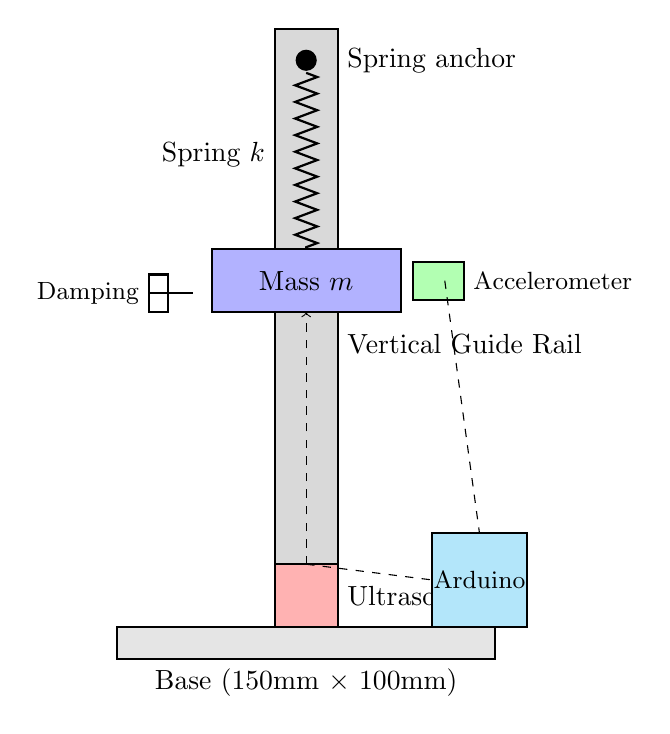
\begin{tikzpicture}[scale=0.8]
% Base
\draw[thick, fill=gray!20] (0,0) rectangle (6,0.5);
\node[below] at (3,0) {Base (150mm $\times$ 100mm)};

% Tower
\draw[thick, fill=gray!30] (2.5,0.5) rectangle (3.5,10);
\node[right] at (3.5,5) {Vertical Guide Rail};

% Spring attachment point
\draw[thick, fill=black] (3,9.5) circle (0.15);
\node[right] at (3.5,9.5) {Spring anchor};

% Spring
\draw[thick, decorate, decoration={zigzag, segment length=6, amplitude=4}]
    (3,9.3) -- (3,6.5);
\node[left] at (2.5,8) {Spring $k$};

% Carriage/Mass
\draw[thick, fill=blue!30] (1.5,5.5) rectangle (4.5,6.5);
\node at (3,6) {Mass $m$};

% Sensor
\draw[thick, fill=green!30] (4.7,5.7) rectangle (5.5,6.3);
\node[right, font=\small] at (5.5,6) {Accelerometer};

% Distance sensor (looking up at mass)
\draw[thick, fill=red!30] (2.5,0.5) rectangle (3.5,1.5);
\node[right] at (3.5,1) {Ultrasonic};
\draw[->, dashed] (3,1.5) -- (3,5.5);

% Damping element (air resistance symbol)
\draw[thick] (1.2,5.8) -- (0.5,5.8);
\draw[thick] (0.5,5.5) rectangle (0.8,6.1);
\node[left, font=\small] at (0.5,5.8) {Damping};

% Arduino
\draw[thick, fill=cyan!30] (5,0.5) rectangle (6.5,2);
\node[font=\small] at (5.75,1.25) {Arduino};

% Connections
\draw[dashed] (5.2,6) -- (5.75,2);
\draw[dashed] (3,1.5) -- (5,1.25);
\end{tikzpicture}
\caption{Experimental apparatus schematic showing the mass-spring-damper assembly with instrumentation.}
\label{fig:apparatus}
\end{figure}

\subsection{Measurement Procedure}

\subsubsection{Static Measurements}

Before dynamic testing, characterize the system parameters statically:

\textbf{1. Spring Constant Measurement:}
\begin{enumerate}
\item Hang the spring vertically with no load. Measure rest length $L_0$.
\item Add known masses incrementally (e.g., 50g, 100g, 150g, 200g).
\item Measure deflection $\delta$ for each mass.
\item Plot force $F = mg$ vs. deflection $\delta$.
\item Spring constant $k = \Delta F / \Delta \delta$ (slope of linear fit).
\end{enumerate}

\textbf{2. Total Mass Measurement:}
\begin{enumerate}
\item Weigh the carriage assembly including accelerometer and wiring.
\item Add washers to achieve desired mass (typically 100--300g total).
\item Record total moving mass $m$.
\end{enumerate}

\subsubsection{Dynamic Measurements: Step Response}

The step response reveals the natural frequency and damping ratio:

\begin{enumerate}
\item Initialize Arduino data logging at 100+ samples/second.
\item Manually displace the mass downward by approximately 20--30mm.
\item Release the mass and record position or acceleration data for 5--10 seconds.
\item Observe the oscillatory decay (if underdamped) or exponential approach (if overdamped).
\end{enumerate}

\textbf{Arduino Code Snippet:}

\begin{lstlisting}[language=C, caption={Arduino code for step response data acquisition}]
#include <Wire.h>

const int trigPin = 9;
const int echoPin = 10;
unsigned long startTime;

void setup() {
    Serial.begin(115200);
    pinMode(trigPin, OUTPUT);
    pinMode(echoPin, INPUT);
    startTime = millis();
}

void loop() {
    // Trigger ultrasonic pulse
    digitalWrite(trigPin, LOW);
    delayMicroseconds(2);
    digitalWrite(trigPin, HIGH);
    delayMicroseconds(10);
    digitalWrite(trigPin, LOW);

    // Measure echo time
    long duration = pulseIn(echoPin, HIGH);
    float distance = duration * 0.034 / 2; // cm

    // Output timestamp and distance
    Serial.print(millis() - startTime);
    Serial.print(",");
    Serial.println(distance);

    delay(10); // 100 Hz sampling
}
\end{lstlisting}

\subsection{Data Analysis and Parameter Extraction}

\subsubsection{Method 1: Logarithmic Decrement}

For an underdamped system, the amplitude decays exponentially while oscillating. The \textbf{logarithmic decrement} $\delta$ is defined as:
\begin{equation}
\delta = \ln\left(\frac{x_n}{x_{n+1}}\right) = \frac{2\pi\zeta}{\sqrt{1-\zeta^2}},
\end{equation}
where $x_n$ and $x_{n+1}$ are successive peak amplitudes.

Solving for damping ratio:
\begin{equation}
\zeta = \frac{\delta}{\sqrt{4\pi^2 + \delta^2}}.
\end{equation}

The \textbf{damped natural frequency} $\omega_d$ is measured from the period of oscillation:
\begin{equation}
\omega_d = \frac{2\pi}{T_d}, \quad \omega_n = \frac{\omega_d}{\sqrt{1-\zeta^2}}.
\end{equation}

\subsubsection{Method 2: Curve Fitting}

The theoretical response to an initial displacement $x_0$ is:
\begin{equation}
x(t) = x_0 e^{-\zeta\omega_n t}\left(\cos\omega_d t + \frac{\zeta}{\sqrt{1-\zeta^2}}\sin\omega_d t\right).
\end{equation}

Using least-squares curve fitting (in MATLAB, Python, or similar), fit this equation to measured data with $\omega_n$ and $\zeta$ as free parameters.

\subsection{Comparing Theory and Experiment}

\textbf{Predicted Parameters:}
\begin{align}
\omega_n^{\text{predicted}} &= \sqrt{k/m} \\
\zeta^{\text{predicted}} &= \frac{b}{2\sqrt{km}}
\end{align}

Note: The damping coefficient $b$ is difficult to measure directly. Friction in the linear guide, air resistance, and internal spring damping all contribute. The experimental measurement of $\zeta$ allows back-calculation of the effective $b$.

\textbf{Expected Results:}

For a typical apparatus with $k \approx 1$ N/mm = 1000 N/m, $m \approx 0.2$ kg:
\begin{equation}
\omega_n = \sqrt{1000/0.2} = 70.7 \text{ rad/s} \approx 11.3 \text{ Hz}.
\end{equation}

With light damping ($\zeta \approx 0.05$ -- 0.1), oscillations should persist for 5--10 cycles before decaying to small amplitude.

\subsection{Sources of Error and Improvements}

\begin{itemize}
\item \textbf{Friction:} Linear guides introduce Coulomb (dry) friction, which is not captured by the viscous damping model. Consider using an air track or magnetic levitation for reduced friction.
\item \textbf{Sensor noise:} Ultrasonic sensors have $\pm$3mm resolution; accelerometers may have offset drift. Averaging and filtering improve results.
\item \textbf{Spring nonlinearity:} Real springs may exhibit nonlinear stiffness at large deflections. Keep oscillation amplitude small (linear region).
\item \textbf{Mass distribution:} The spring itself has mass that oscillates; this adds approximately $1/3$ of the spring mass to the effective moving mass.
\end{itemize}


\section{Worked Examples}

\subsection{Example 1: Simple Pendulum}

\textbf{Problem:} Derive the equation of motion for a simple pendulum consisting of a point mass $m$ at the end of a massless rod of length $\ell$.

\textbf{Solution:}

\begin{figure}[htbp]
\centering
\begin{tikzpicture}[scale=1.2]
% Pivot
\fill (0,0) circle (0.08);
\draw[thick] (-0.3,0.1) -- (0.3,0.1);
\draw[pattern=north east lines] (-0.3,0.1) rectangle (0.3,0.25);

% Rod
\draw[thick] (0,0) -- (2,-2.5);
\node[right] at (1,-1.25) {$\ell$};

% Mass
\fill[blue] (2,-2.5) circle (0.2);
\node[right] at (2.3,-2.5) {$m$};

% Angle
\draw[dashed] (0,0) -- (0,-2);
\draw[->, thick] (0,-1) arc (-90:-52:1);
\node[below] at (0.3,-0.8) {$\theta$};

% Forces on mass (FBD)
\draw[->, thick, red] (2,-2.5) -- (2,-4);
\node[right, red] at (2,-3.5) {$mg$};
\draw[->, thick, blue] (2,-2.5) -- (0.7,-1.35);
\node[left, blue] at (1,-1.8) {$T$};

% Tangential direction
\draw[->, thick, green!50!black] (2,-2.5) -- (3.2,-1.9);
\node[above, green!50!black] at (3,-2) {$\hat{e}_{\theta}$};
\end{tikzpicture}
\caption{Simple pendulum geometry and free body diagram.}
\label{fig:pendulum}
\end{figure}

Using polar coordinates centered at the pivot, the tangential component of Newton's Second Law gives:
\begin{equation}
m\ell\ddot{\theta} = -mg\sin\theta.
\end{equation}

Thus:
\begin{equation}
\boxed{\ddot{\theta} + \frac{g}{\ell}\sin\theta = 0}
\end{equation}

This is a \textbf{nonlinear} differential equation due to the $\sin\theta$ term.

\textbf{Linearization for Small Angles:}

For small angles, $\sin\theta \approx \theta$, yielding:
\begin{equation}
\ddot{\theta} + \frac{g}{\ell}\theta = 0.
\end{equation}

This is simple harmonic motion with natural frequency:
\begin{equation}
\omega_n = \sqrt{g/\ell}.
\end{equation}

For $\ell = 1$ m: $\omega_n = \sqrt{9.81/1} = 3.13$ rad/s, corresponding to period $T = 2\pi/\omega_n = 2.01$ s.

\hrulefill

\subsection{Example 2: DC Motor Model}

\textbf{Problem:} Derive the transfer function from applied voltage $V(s)$ to motor shaft angular velocity $\Omega(s)$ for a DC motor.

\textbf{Solution:}

A DC motor couples electrical and mechanical domains. The relevant equations are:

\textbf{Electrical (armature circuit):}
\begin{equation}
V = L_a\frac{di_a}{dt} + R_a i_a + e_b,
\end{equation}
where $e_b = K_b\omega$ is the back-EMF (proportional to angular velocity).

\textbf{Mechanical (rotor):}
\begin{equation}
J\frac{d\omega}{dt} + b\omega = \tau_m = K_t i_a,
\end{equation}
where $K_t$ is the torque constant and for a DC motor, $K_t = K_b = K$ (motor constant).

\textbf{State-Space Form:}

Defining states $\mathbf{x} = [i_a, \omega]^T$:
\begin{equation}
\begin{bmatrix} \dot{i}_a \\ \dot{\omega} \end{bmatrix} =
\begin{bmatrix} -R_a/L_a & -K/L_a \\ K/J & -b/J \end{bmatrix}
\begin{bmatrix} i_a \\ \omega \end{bmatrix} +
\begin{bmatrix} 1/L_a \\ 0 \end{bmatrix} V.
\end{equation}

\textbf{Transfer Function:}

Taking Laplace transforms (with zero initial conditions):
\begin{align}
V(s) &= (L_a s + R_a)I_a(s) + K\Omega(s) \\
(Js + b)\Omega(s) &= KI_a(s).
\end{align}

Solving for $\Omega(s)/V(s)$:
\begin{equation}
\boxed{\frac{\Omega(s)}{V(s)} = \frac{K}{(L_a s + R_a)(Js + b) + K^2} = \frac{K}{L_a J s^2 + (L_a b + R_a J)s + (R_a b + K^2)}}
\end{equation}

For many motors, $L_a$ is small enough to neglect, yielding a first-order approximation:
\begin{equation}
\frac{\Omega(s)}{V(s)} \approx \frac{K/R_a}{(JR_a/(R_ab + K^2))s + 1} = \frac{K_m}{\tau_m s + 1},
\end{equation}
where $K_m = K/(R_ab + K^2)$ is the motor gain and $\tau_m = JR_a/(R_ab + K^2)$ is the mechanical time constant.

\hrulefill

\subsection{Example 3: Finding Natural Frequency and Damping Ratio}

\textbf{Problem:} A mass-spring-damper system has $m = 2$ kg, $k = 200$ N/m, and $b = 8$ N$\cdot$s/m. Find $\omega_n$, $\zeta$, and classify the system response.

\textbf{Solution:}

\begin{align}
\omega_n &= \sqrt{k/m} = \sqrt{200/2} = 10 \text{ rad/s} \\
\zeta &= \frac{b}{2\sqrt{km}} = \frac{8}{2\sqrt{200 \cdot 2}} = \frac{8}{2 \cdot 20} = 0.2
\end{align}

Since $0 < \zeta < 1$, the system is \textbf{underdamped} and will exhibit oscillatory decay.

The damped natural frequency is:
\begin{equation}
\omega_d = \omega_n\sqrt{1-\zeta^2} = 10\sqrt{1-0.04} = 9.80 \text{ rad/s}.
\end{equation}

The oscillation period is $T_d = 2\pi/\omega_d = 0.641$ s.

\hrulefill

\subsection{Example 4: Fluid Tank Level Control}

\textbf{Problem:} Derive the differential equation governing the liquid level $h$ in a tank with cross-sectional area $A$, inlet flow rate $q_{\text{in}}(t)$, and outlet flow through a resistance $R$ (where flow is proportional to pressure drop).

\begin{figure}[htbp]
\centering
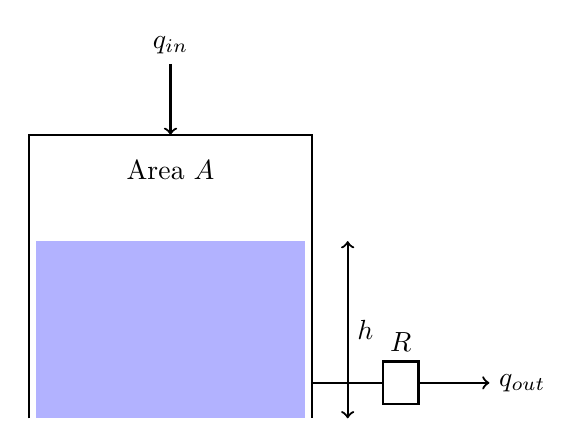
\begin{tikzpicture}[scale=0.9]
% Tank
\draw[thick] (0,0) -- (0,4) -- (4,4) -- (4,0);
% Water
\fill[blue!30] (0.1,0) rectangle (3.9,2.5);
% Water level indicator
\draw[<->, thick] (4.5,0) -- (4.5,2.5);
\node[right] at (4.5,1.25) {$h$};
% Inlet
\draw[thick, ->] (2,5) -- (2,4);
\node[above] at (2,5) {$q_{\text{in}}$};
% Outlet with resistance
\draw[thick] (4,0.5) -- (5,0.5);
\draw[thick] (5,0.2) rectangle (5.5,0.8);
\node[above] at (5.25,0.8) {$R$};
\draw[thick, ->] (5.5,0.5) -- (6.5,0.5);
\node[right] at (6.5,0.5) {$q_{\text{out}}$};
% Area label
\node at (2,3.5) {Area $A$};
\end{tikzpicture}
\caption{Tank level control system schematic.}
\label{fig:tank}
\end{figure}

\textbf{Solution:}

\textbf{Conservation of Mass:}
\begin{equation}
\frac{d(\rho V)}{dt} = \rho q_{\text{in}} - \rho q_{\text{out}},
\end{equation}
where $V = Ah$ is the liquid volume. For incompressible fluid:
\begin{equation}
A\frac{dh}{dt} = q_{\text{in}} - q_{\text{out}}.
\end{equation}

\textbf{Outlet Flow Relationship:}

The outlet flow is driven by hydrostatic pressure $\rho g h$. For a linear resistance:
\begin{equation}
q_{\text{out}} = \frac{\rho g h}{R}.
\end{equation}

\textbf{Final Equation:}
\begin{equation}
A\frac{dh}{dt} + \frac{\rho g}{R}h = q_{\text{in}}.
\end{equation}

Defining the time constant $\tau = AR/(\rho g)$:
\begin{equation}
\boxed{\tau\frac{dh}{dt} + h = \frac{R}{\rho g}q_{\text{in}}}
\end{equation}

This is a first-order system. The steady-state level for constant inlet flow $q_{\text{in}} = Q$ is:
\begin{equation}
h_{\text{ss}} = \frac{RQ}{\rho g}.
\end{equation}

\hrulefill

\subsection{Example 5: Coupled Mass-Spring System}

\textbf{Problem:} Two masses $m_1$ and $m_2$ are connected by springs as shown. Derive the equations of motion.

\begin{figure}[htbp]
\centering
\begin{tikzpicture}[scale=0.9]
% Ground
\fill[pattern=north east lines] (-0.5,0) rectangle (0,2);
\draw[thick] (0,0) -- (0,2);

% Spring 1
\draw[thick, decorate, decoration={zigzag, segment length=5, amplitude=3}]
    (0,1) -- (2,1);
\node[above] at (1,1.3) {$k_1$};

% Mass 1
\draw[thick, fill=gray!30] (2,0.5) rectangle (3.5,1.5);
\node at (2.75,1) {$m_1$};

% Spring 2
\draw[thick, decorate, decoration={zigzag, segment length=5, amplitude=3}]
    (3.5,1) -- (5.5,1);
\node[above] at (4.5,1.3) {$k_2$};

% Mass 2
\draw[thick, fill=gray!30] (5.5,0.5) rectangle (7,1.5);
\node at (6.25,1) {$m_2$};

% Positions
\draw[<->] (2.75,-0.2) -- (2.75,-0.8);
\node[below] at (2.75,-0.8) {$x_1$};
\draw[<->] (6.25,-0.2) -- (6.25,-0.8);
\node[below] at (6.25,-0.8) {$x_2$};
\end{tikzpicture}
\caption{Two-mass coupled oscillator system.}
\label{fig:coupled_mass}
\end{figure}

\textbf{Solution:}

\textbf{Free Body Diagram for $m_1$:}
\begin{itemize}
\item Force from spring $k_1$: $-k_1 x_1$ (restoring toward wall)
\item Force from spring $k_2$: $k_2(x_2 - x_1)$ (depends on relative displacement)
\end{itemize}

\textbf{Free Body Diagram for $m_2$:}
\begin{itemize}
\item Force from spring $k_2$: $-k_2(x_2 - x_1)$
\end{itemize}

\textbf{Equations of Motion:}
\begin{align}
m_1\ddot{x}_1 &= -k_1 x_1 + k_2(x_2 - x_1) \\
m_2\ddot{x}_2 &= -k_2(x_2 - x_1)
\end{align}

\textbf{Matrix Form:}
\begin{equation}
\begin{bmatrix} m_1 & 0 \\ 0 & m_2 \end{bmatrix}
\begin{bmatrix} \ddot{x}_1 \\ \ddot{x}_2 \end{bmatrix} +
\begin{bmatrix} k_1 + k_2 & -k_2 \\ -k_2 & k_2 \end{bmatrix}
\begin{bmatrix} x_1 \\ x_2 \end{bmatrix} =
\begin{bmatrix} 0 \\ 0 \end{bmatrix}
\end{equation}

Or more compactly:
\begin{equation}
\boxed{\mathbf{M}\ddot{\mathbf{x}} + \mathbf{K}\mathbf{x} = \mathbf{0}}
\end{equation}

This system has two natural frequencies (normal modes), found by solving the eigenvalue problem:
\begin{equation}
\det(\mathbf{K} - \omega^2\mathbf{M}) = 0.
\end{equation}


\section{Chapter Summary}

This chapter established the foundation for all subsequent control system analysis: the mathematical model. Key concepts include:

\begin{enumerate}
\item \textbf{Historical Context:} Mathematical modeling of physical systems evolved from Newton's mechanics (1687) through Kirchhoff's circuit laws (1845) to Heaviside's operational calculus (1880s), driven by practical needs in astronomy, telegraphy, and engineering.

\item \textbf{The Modeling Process:} Apply physical laws (conservation of energy, momentum, charge) combined with constitutive relationships (Hooke's Law, Ohm's Law, etc.) to derive differential equations.

\item \textbf{The Mass-Spring-Damper Paradigm:} The equation $m\ddot{x} + b\dot{x} + kx = F(t)$ appears across mechanical, electrical, thermal, and other domains through appropriate analogies.

\item \textbf{Standard Form:} Second-order systems are characterized by natural frequency $\omega_n$ and damping ratio $\zeta$, which determine dynamic response.

\item \textbf{System Order:} The order of the differential equation equals the number of independent energy storage elements.

\item \textbf{Experimental Validation:} Physical models must be validated against real measurements. Discrepancies reveal unmodeled dynamics or parameter uncertainty.
\end{enumerate}

\section{Problems}

\begin{enumerate}
\item A mass $m = 0.5$ kg is suspended from a spring with stiffness $k = 50$ N/m and viscous damper with coefficient $b = 2$ N$\cdot$s/m.
\begin{enumerate}
    \item Derive the equation of motion.
    \item Find the natural frequency and damping ratio.
    \item Classify the response as overdamped, critically damped, or underdamped.
    \item If the mass is displaced 5 cm and released, estimate the time for oscillations to decay to 1 cm amplitude.
\end{enumerate}

\item For the series RLC circuit with $R = 100\ \Omega$, $L = 0.1$ H, and $C = 10\ \mu$F:
\begin{enumerate}
    \item Derive the differential equation for capacitor voltage.
    \item Find the natural frequency and damping ratio.
    \item Sketch the expected response to a step input voltage.
\end{enumerate}

\item A thermal system consists of a heated metal block (mass 1 kg, specific heat 500 J/(kg$\cdot$K)) in an insulated enclosure with a small air gap providing thermal resistance $R_{\text{th}} = 2$ K/W to ambient.
\begin{enumerate}
    \item Derive the differential equation relating block temperature to heater power.
    \item Find the thermal time constant.
    \item If the heater provides 50 W and ambient is 20$^\circ$C, what is the steady-state block temperature?
\end{enumerate}

\item Design an experiment to measure the moment of inertia of a flywheel using only a stopwatch and known applied torque. Derive the relevant equations and describe the procedure.

\item For the tank level system of Example 4, the tank has cross-sectional area $A = 1$ m$^2$, and water exits through an orifice with effective resistance such that $q_{\text{out}} = 0.1\sqrt{h}$ m$^3$/s (nonlinear).
\begin{enumerate}
    \item Linearize the outlet flow relationship about an operating point $h_0 = 1$ m.
    \item Find the linearized time constant.
    \item Compare the linear and nonlinear responses to a small step change in inlet flow.
\end{enumerate}

\item Using the Lagrangian method, derive the equations of motion for a double pendulum (two point masses connected by two massless rods). You need not solve the resulting equations.

\item A DC motor has the following parameters: $R_a = 2\ \Omega$, $L_a = 5$ mH, $K = 0.1$ V$\cdot$s/rad = 0.1 N$\cdot$m/A, $J = 0.01$ kg$\cdot$m$^2$, $b = 0.001$ N$\cdot$m$\cdot$s/rad.
\begin{enumerate}
    \item Write the state-space model with states $[i_a, \omega]^T$.
    \item Find the transfer function from voltage to angular velocity.
    \item Determine if the electrical time constant is small enough to justify the first-order approximation.
\end{enumerate}
\end{enumerate}


\section{Further Reading}

\begin{itemize}
\item Cannon, R.H., \textit{Dynamics of Physical Systems}, McGraw-Hill, 1967. A classic text on deriving equations of motion from physical principles.
\item Shearer, J.L., Murphy, A.T., and Richardson, H.H., \textit{Introduction to System Dynamics}, Addison-Wesley, 1967. Excellent treatment of analogies between domains.
\item Ogata, K., \textit{System Dynamics}, 4th ed., Pearson, 2003. Comprehensive coverage with many worked examples.
\item Heaviside, O., \textit{Electromagnetic Theory}, 1893. The original source for operational calculus; historically fascinating if mathematically challenging.
\end{itemize}

\end{chapter}
